\documentclass[12pt]{article}
\usepackage[utf8]{inputenc, }
\usepackage{graphicx}
\usepackage{hyperref}
\usepackage[margin=1in]{geometry}
\usepackage{setspace}
\usepackage{color}
\usepackage{pdfpages}
\usepackage{amsmath}
\usepackage{amsfonts}
\usepackage{float}
\usepackage{tikz}
\usepackage{pgfplots}
\usepackage{enumitem}
\usepackage{xpatch}
\usepackage{svg}
\usepackage{mathrsfs}
\usepackage{steinmetz}
% \usepackage[nocheck]{fancyhdr}

\sloppy
\definecolor{lightgray}{gray}{0.5}
\setlength{\parindent}{0pt}

\hypersetup{
    colorlinks,
    citecolor=black,
    filecolor=black,
    linkcolor=black,
    urlcolor=black
    pdftitle={EE300 İsmail Enes Bülbül}
}
\onehalfspacing

% \raggedright

\title{EE301 Homework-4}
\author{İsmail Enes Bülbül, Eren Meydanlı, Ahmet Caner Akar}
%\date{October 2022}
\renewcommand*\contentsname{Table of Contents}
\renewcommand*{\refname}{}
% \fancyhf{} % sets both header and footer to nothing
% \renewcommand{\headrulewidth}{0pt}
\begin{document}

\maketitle
% \tableofcontents
% \newpage

    \section*{Question 1}
    \subsection*{a)}
    \begin{math} 
    x_s(t) = x(t) s(t) = \displaystyle\sum_{n=-\infty}^{\infty} x(t) \delta(t-nT_s) = \displaystyle\sum_{n=-\infty}^{\infty} x(nT_s) \delta(t-nT_s)\\ 
    \textrm{where } T_s \textrm{ is called the sampling period.}\\
    \textrm{By the modulation property of CTFT: } X_s(j\omega) = \frac{1}{2\pi} X(j\omega)*S(j\omega) \\ \\
    \textrm{s(t) is a periodic signal, therefore we should first find its CTFS representation: }\\
    s(t) = \displaystyle\sum_{k=-\infty}^{\infty} a_k e^{jk\omega_s t}, \omega_s = \frac{2\pi}{T_s} \\
    a_k = \frac{1}{T_s} \displaystyle\int_{-T_s/2}^{T_s/2} \underbrace{s(t)}_{\delta(t)} e^{-jk\omega_s t} dt \Rightarrow a_k = \frac{1}{T_s} \\
    s(t) = \displaystyle\sum_{k=-\infty}^{\infty} \frac{1}{T_s} e^{jk\omega_s t} \longrightarrow S(j\omega) = \displaystyle\sum_{k=-\infty}^{\infty} \frac{2\pi}{T_s} \delta(\omega-k\omega_s) \\ \\
    X_s(j\omega) = \frac{1}{2\pi} X(j\omega)*\displaystyle\sum_{k=-\infty}^{\infty} \frac{2\pi}{T_s} \delta(\omega-k\omega_s) = \displaystyle\sum_{k=-\infty}^{\infty} \frac{1}{T_s} X(j(\omega-k\omega_s)) 
    \end{math} \\ \\
    From the Nyquist sampling theorem, the inequality \(\omega_s \geq 2\Delta\omega\) should be satisfied so that the shifted replicas of \(X(j\omega)\) do not overlap. Thus, it yields perfect reconstruction of the signal \(x(t)\) from \(x_s(t)\) with no aliasing. So, the minumum sampling rate, \(\omega_s = 2\Delta\omega\). The Fourier transform of the sampling system output, \(X_s(j\omega)\) can be seen below. \\ 
     \begin{center}
  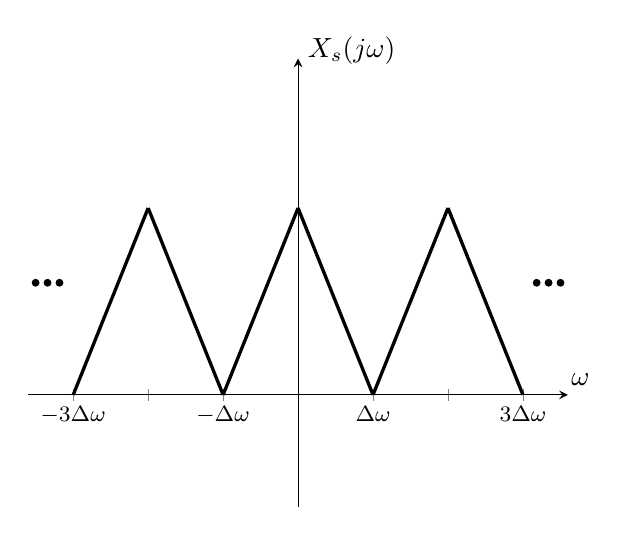
\begin{tikzpicture}
\begin{axis}[
    axis lines = middle,
    ymin = -0.2,
    ymax = 0.8,
    xlabel = \(\omega\),
    xlabel style={xshift=0.4cm},
    ylabel style={yshift=0.4cm},
    ylabel = {\(X_s(j\omega)\)},
    xtick={-3*pi, -2*pi, -1*pi, 0, 1*pi, 2*pi, 3*pi},
    xticklabel style={font=\footnotesize,fill=white,inner sep=2pt},
    xticklabels={$-3\Delta\omega$,,$-\Delta\omega$,,$\Delta\omega$,,$3\Delta\omega$},
    samples=500,
    enlargelimits=true,
    ytick style={draw=none},
    yticklabels={draw=none},
    ]
       \addplot [domain=-1*pi:0,style=very thick,black] {(x+pi)/(2*pi)};
       \addplot [domain=0:1*pi,style=very thick,black] {(pi-x)/(2*pi)};
       \addplot [domain=-2*pi:-1*pi,style=very thick,black] {-(x+pi)/(2*pi)};
       \addplot [domain=-3*pi:-2*pi,style=very thick,black] {(x+3*pi)/(2*pi)};
       \addplot [domain=1*pi:2*pi,style=very thick,black] {(x-pi)/(2*pi)};
       \addplot [domain=2*pi:3*pi,style=very thick,black] {-(x-3*pi)/(2*pi)};
       \filldraw[black] (axis cs: 10,0.3) circle (1.2pt) node[anchor=west]{};
        \filldraw[black] (axis cs: 10.5,0.3) circle (1.2pt) node[anchor=west]{};
        \filldraw[black] (axis cs: 11,0.3) circle (1.2pt) node[anchor=west]{};
        \filldraw[black] (axis cs: -10,0.3) circle (1.2pt) node[anchor=west]{};
        \filldraw[black] (axis cs: -10.5,0.3) circle (1.2pt) node[anchor=west]{};
        \filldraw[black] (axis cs: -11,0.3) circle (1.2pt) node[anchor=west]{};
\end{axis}
\end{tikzpicture}
\end{center}
    
    \subsection*{b)}
    \(X(j\omega)\) is not symmetric with respect to y-axis, thus from the symmetry property of CTFT it can be concluded that \(x(t)\) is a complex-valued signal. 
    \subsubsection*{i)}
    Since the sampling rate of the signal is equal to the Nyquist rate, the aliasing does not occur. The Fourier transform of \(X_s(j\omega)\) is plotted below for \( T_s = \frac{\pi}{\Delta\omega}\). 
         \begin{center}
  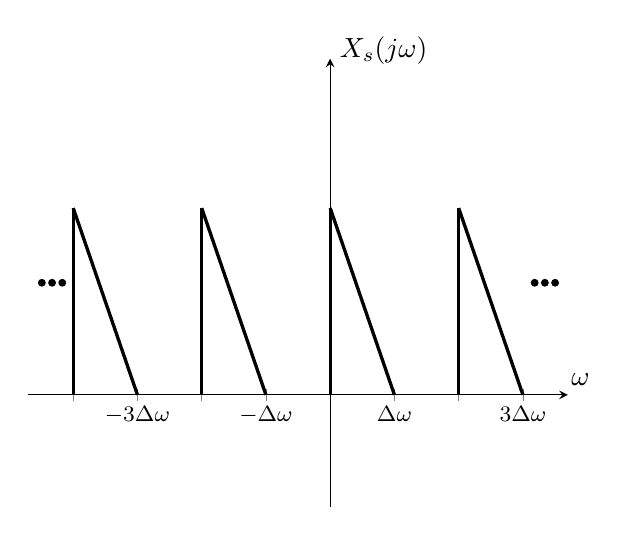
\begin{tikzpicture}
\begin{axis}[
    axis lines = middle,
    ymin = -0.2,
    ymax = 0.8,
    xlabel = \(\omega\),
    xlabel style={xshift=0.4cm},
    ylabel style={yshift=0.4cm},
    ylabel = {\(X_s(j\omega)\)},
    xtick={-4*pi,-3*pi, -2*pi, -1*pi, 0, 1*pi, 2*pi, 3*pi},
    xticklabel style={font=\footnotesize,fill=white,inner sep=2pt},
    xticklabels={,$-3\Delta\omega$,,$-\Delta\omega$,,$\Delta\omega$,,$3\Delta\omega$},
    samples=500,
    enlargelimits=true,
    ytick style={draw=none},
    yticklabels={draw=none},
    ]
       \addplot [domain=0:1*pi,style=very thick,black] {(pi-x)/(2*pi)};
       \addplot [domain=-2*pi:-pi,style=very thick,black] {-(x+pi)/(2*pi)};
       \addplot [domain=2*pi:3*pi,style=very thick,black] {-(x-3*pi)/(2*pi)};
       \addplot [domain=-4*pi:-3*pi,style=very thick,black] {-(x+3*pi)/(2*pi)};
       \filldraw[black] (axis cs: 10,0.3) circle (1.2pt) node[anchor=west]{};
        \filldraw[black] (axis cs: 10.5,0.3) circle (1.2pt) node[anchor=west]{};
        \filldraw[black] (axis cs: 11,0.3) circle (1.2pt) node[anchor=west]{};
        \filldraw[black] (axis cs: -13.1,0.3) circle (1.2pt) node[anchor=west]{};
        \filldraw[black] (axis cs: -13.6,0.3) circle (1.2pt) node[anchor=west]{};
        \filldraw[black] (axis cs: -14.1,0.3) circle (1.2pt) node[anchor=west]{};
        \draw[very thick] (axis cs: -2*pi,0)--(axis cs: -2*pi,0.5);
        \draw[very thick] (axis cs: -4*pi,0)--(axis cs: -4*pi,0.5);
        \draw[very thick] (axis cs: 0,0)--(axis cs: 0,0.5);
        \draw[very thick] (axis cs: 2*pi,0)--(axis cs: 2*pi,0.5);
\end{axis}
\end{tikzpicture}
\end{center}
    \subsubsection*{ii)}
    As it can be seen from the graph of the Fourier transform of \(x(t)\), the graph is not symmetric with respect to y-axis, i.e., \(X(j\omega)\) has no component at negative frequencies. Therefore, as it can be seen from the graph of \(X_s(j\omega)\) below, the aliasing can be avoided even when \(T_s = \frac{2\pi}{\Delta\omega}\) which below the Nyquist rate. 
   \begin{center}
  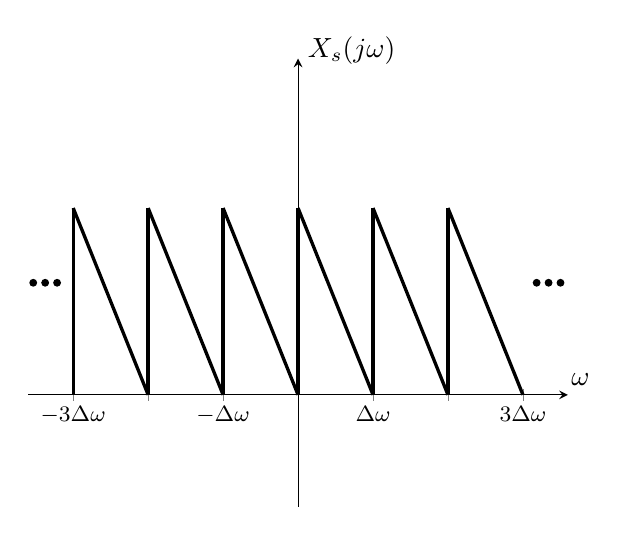
\begin{tikzpicture}
\begin{axis}[
    axis lines = middle,
    ymin = -0.2,
    ymax = 0.8,
    xlabel = \(\omega\),
    xlabel style={xshift=0.4cm},
    ylabel style={yshift=0.4cm},
    ylabel = {\(X_s(j\omega)\)},
    xtick={-3*pi, -2*pi, -1*pi, 0, 1*pi, 2*pi, 3*pi},
    xticklabel style={font=\footnotesize,fill=white,inner sep=2pt},
    xticklabels={$-3\Delta\omega$,,$-\Delta\omega$,,$\Delta\omega$,,$3\Delta\omega$},
    samples=500,
    enlargelimits=true,
    ytick style={draw=none},
    yticklabels={draw=none},
    ]
       \addplot [domain=0:1*pi,style=very thick,black] {(pi-x)/(2*pi)};
       \addplot [domain=pi:2*pi,style=very thick,black] {-(x-2*pi)/(2*pi)};
       \addplot [domain=-pi:0,style=very thick,black] {(-x)/(2*pi)};
       \addplot [domain=-2*pi:-pi,style=very thick,black] {-(x+pi)/(2*pi)};
       \addplot [domain=-3*pi:-2*pi,style=very thick,black] {-(x+2*pi)/(2*pi)};
       \addplot [domain=2*pi:3*pi,style=very thick,black] {-(x-3*pi)/(2*pi)};
       \filldraw[black] (axis cs: 10,0.3) circle (1.2pt) node[anchor=west]{};
        \filldraw[black] (axis cs: 10.5,0.3) circle (1.2pt) node[anchor=west]{};
        \filldraw[black] (axis cs: 11,0.3) circle (1.2pt) node[anchor=west]{};
        \filldraw[black] (axis cs: -10.1,0.3) circle (1.2pt) node[anchor=west]{};
        \filldraw[black] (axis cs: -10.6,0.3) circle (1.2pt) node[anchor=west]{};
        \filldraw[black] (axis cs: -11.1,0.3) circle (1.2pt) node[anchor=west]{};
        \draw[very thick] (axis cs: -2*pi,0)--(axis cs: -2*pi,0.5);
        \draw[very thick] (axis cs: -3*pi,0)--(axis cs: -3*pi,0.5);
        \draw[very thick] (axis cs: -pi,0)--(axis cs: -pi,0.5);
        \draw[very thick] (axis cs: pi,0)--(axis cs: pi,0.5);
        \draw[very thick] (axis cs: 0,0)--(axis cs: 0,0.5);
        \draw[very thick] (axis cs: 2*pi,0)--(axis cs: 2*pi,0.5);
\end{axis}
\end{tikzpicture}
\end{center}

    \subsection*{c)}
    
    \section*{Question 2}
    \subsection*{i)}
    
    \subsection*{ii)}
    
    \section*{Question 3}
    \subsection*{a)}
    
    \subsection*{b)}
     \subsubsection*{i)}       
    
    \subsubsection*{ii)}
    
     \subsubsection*{iii)}
    
     \subsection*{c)}
     \subsubsection*{i)}       
    
    \subsubsection*{ii)}
    
     \subsection*{d)}
     \subsubsection*{i)}       
    
    \subsubsection*{ii)}
    
     \subsubsection*{iii)}
       
     \section*{Question 4}
     \subsection*{a)}
    
     \subsection*{b)}
    
     \subsection*{c)}
    
     \subsection*{d)}     
    
\end{document}